% =====================================================================
%  Paper template — AASTeX v7, two-column
%  Wide figures span both columns via figure* (text flows above/below;
%  LaTeX two-column has no text-wrap around full-width floats)
%
%  Build:  pdflatex paper_template.tex   (run twice for references/labels)
%  Requires the AASTeX class. TeX Live ships it as `aastex701` (v7.0.1),
%  which is what this template uses and what AAS now recommends.
%  If not installed:  tlmgr install aastex
%
%  NOTE: your RNAA draft was typeset with the older `aastex631` (v6.31).
%  If a journal specifically requires v6.31, change the class below to
%  aastex631 and install it (Overleaf has both; local TeX Live ships v7).
%  The two-column look is the same either way.
% =====================================================================

% ---- Class options ---------------------------------------------------
%   twocolumn : dense two-column journal layout. Wide multi-panel
%               figures use figure* (spans BOTH columns, full text
%               width); single-panel figures stay at \columnwidth.
%   Alternatives:
%     [modern]      -> single column, wider, cleaner for reading
%     [manuscript]  -> double-spaced single column, for refereeing
% ---------------------------------------------------------------------
\documentclass[twocolumn]{aastex701}

% ---- Packages --------------------------------------------------------
\usepackage{amsmath}        % \eqref, align; safe to keep with aastex
\usepackage{xcolor}         % kept for draft markup (no colored text at present)
\usepackage{etoolbox}       % \patchcmd, used for heading spacing below
% \usepackage{physics}      % \dv, \pdv, \abs, ... (not on all systems)

% ---- Heading whitespace ----------------------------------------------
% AASTeX packs headings tight (9pt above / 4pt below). Loosen to a more
% book-like rhythm (abnTeX2-style airiness): ~2 blank lines above a
% section, ~1 below; slightly less for subsections. Only the two spacing
% arguments of \@startsection are patched; numbering/fonts are untouched.
\makeatletter
\patchcmd{\section}{{9pt plus 1pt minus 1pt}{4pt}}%
                   {{28pt plus 6pt minus 2pt}{14pt plus 2pt}}{}{%
  \typeout{WARNING: \string\section\space spacing patch failed}}
\patchcmd{\subsection}{{9pt plus 1pt minus 1pt}{4pt}}%
                      {{20pt plus 4pt minus 2pt}{10pt plus 2pt}}{}{%
  \typeout{WARNING: \string\subsection\space spacing patch failed}}
\makeatother

% ---- Convenience macros ----------------------------------------------
\newcommand{\msun}{M_\odot}
\newcommand{\rns}{R_{\rm NS}}
\newcommand{\code}[1]{\texttt{#1}}

% ---- Running-head metadata (top of every page) -----------------------
\shorttitle{The Systematic in the isotropic assumption}
\shortauthors{Panchal \& ud-Doula}

% ---- Optional: where \includegraphics looks for figures --------------
% Drafting: pull figures straight from data/. For submission, regenerate
% at >= 600 dpi into figures/ and switch this path.
\graphicspath{{../../data/}{./figures/}{./}}  % data/ locally; figures/ on Overleaf; ./ for local images

\begin{document}

% =====================================================================
%  TITLE BLOCK
% =====================================================================
\title{The Systematic in the isotropic assumption for Neutron stars}

% --- Authors and affiliations (headers copied from docs/RNAA_draft.pdf) ---
% AASTeX v7 REQUIRES every \author to have its own \affiliation AND \email.
% The @example.edu emails are placeholders -> replace with institutional ones.
\author{Ameya Panchal}
\affiliation{Penn State University, University Park, PA, USA}
\email{avp6407@psu.edu}

\author{Asif ud-Doula}
\affiliation{Penn State Scranton, Dunmore, PA, USA}
\email{auu4@psu.edu}

\correspondingauthor{Ameya Panchal}

% =====================================================================
%  ABSTRACT — MDPI: max ~200 words, single paragraph, implicitly
%  structured background -> methods -> results -> conclusion.
% =====================================================================
\begin{abstract}
Pulsed-fraction and pulse-profile analyses of X-ray hot spots on rotating neutron stars
underpin their mass--radius measurements. However, simplified and exploratory pulse-profile
work can assume isotropic surface emission for simplicity.
We quantify the systematic (in assuming isotropic beaming vs realistic beaming) introduced,
in various star conditions, including published NICER geometries for J0740+6620 and
J0030+0451. 
To do this, we generate a beaming function through a Monte Carlo scattering atmosphere, and
feed into general-relativistic pulse profiles with Schwarzschild light bending and Doppler
effects. 
This was validated against Chandrasekhar's H function and Bogdanov et al. reference
waveforms. We then construct two pulse profile graphs, swapping the MC emission with
isotropic emission, to compute the pulse-profile and pulsed-fraction analyses. 
The systematic reaches +0.14/+0.20 in pulsed fraction (static, bolometric), draining to
+0.02/+0.07 at the real spin (convention- and band-dependent), while a waveform-shape difference of
$\approx 0.10$ RMS (peak-normalized) persists nearly unchanged across spin. The most
intriguing find is that azimuthal separation and spin route the systematic between
pulsed-fraction and waveform shape.
Additionally, when summed multi-spot flux hits zero, the systematic can hide it entirely
from the pulsed-fraction, leaving only the waveform shape.
These numbers quantify what the isotropy shortcut costs simplified and exploratory
pulse-profile work; the flagship NICER inferences fit beamed model atmospheres and are not
the target of this systematic. The systematic never vanishes, it only moves outside
measurement.
\end{abstract}

% ---- Keywords — MDPI requires 3–10 (specific but discipline-common) --
\keywords{neutron stars --- pulsars: individual (PSR J0740$+$6620, PSR J0030$+$0451) ---
radiative transfer --- Monte Carlo methods --- X-rays: stars}

% =====================================================================
%  BODY
% =====================================================================

\section{Introduction} \label{sec:intro}
Pulse-profile modeling has enabled precise constraints on neutron star masses and radii
\citep{Bogdanov2019, Riley2019, Miller2019}.
A key systematic uncertainty in these analyses is the assumed angular distribution of
emergent radiation from surface hot spots. Most simplified and exploratory models adopt
isotropic or parameterized limb-darkening laws
\citep[e.g.][]{AnnalaPoutanen2010,Psaltis2014,Sotani2018}.
The full NICER inference pipelines themselves fit beamed hydrogen-atmosphere models rather
than isotropic emission \citep{Bogdanov2019,Riley2019,Miller2019}; the systematic quantified
here is therefore the cost of the isotropy shortcut in that simplified tier of analyses, not
a bias in the published mass--radius posteriors.
Previous studies include \citet{Zhao2024a, Zhao2024b} and \citet{Baubock2015}, which analyze
how a wrong beaming function and hotspot size biases inferred radius respectively, but do
not address azimuthal separation, hot-spot tiling, or pulsed fraction as we do.
In this paper, we observe a systematic between isotropic beaming and realistic beaming, and
quantify it through pulsed fraction. We also observe how azimuthal separation and high spin
influence this systematic.
Additionally, through azimuthal separation, we observe a rule determining if the systematic
shows in the pulsed fraction at all: if the summed flux of all hotspots never touches zero
(the spots \emph{tile} the rotation), the pulsed fraction stays live; if it does touch zero,
the pulsed fraction saturates at 1 and the systematic hides in the waveform shape instead.
Section~\ref{sec:methods} describes the pipeline and its validation,
Section~\ref{sec:results} presents the results at the two NICER anchors and across geometry
and spin, and Section~\ref{sec:discussion} discusses limitations and implications.

\section{Methods} \label{sec:methods}
Overall, this is a two-part pipeline. The Monte Carlo scattering atmosphere generates the
beaming function $I(\mu;\tau)$, which returns intensity based on the cosine of the emission
angle. This is then fed directly into the deterministic pulse machinery. The paper's central
number, the change in pulsed fraction between the realistic and isotropic runs, is defined
at the end of this section (Equation~\eqref{eq:dpf}).


\subsection{Monte Carlo Scattering Atmosphere} \label{sec:methods-mc}
The Monte Carlo scattering atmosphere contains the only stochastic elements of this
experiment. The transport engine can be explained as an equally bright (Lambertian) thermal
source: because a surface element's projected area scales as $\mu = \cos\theta$, an equally
bright source sends photon \emph{counts} across the base as $N(\mu) \propto \mu$, not
equally in every direction.
As such, initial photon emission angles must be sampled from
\begin{equation}
    \cos\theta_0 = \sqrt{U}, \label{eq:injection}
\end{equation}
where $U$ is a uniform random deviate; sampling $\cos\theta_0$ uniformly would instead
over-produce grazing photons \citep{Cashwell1959,Whitney2011}. These photons are injected at
the base of a plane-parallel, horizontally-infinite atmosphere. The base is a perfect
absorber (a photon that random-walks back down is lost) so the beaming function measured
here is the \emph{transmission} beaming of a passive scattering layer, we are only measuring
escapes.
The vertical thickness of the atmosphere is its total optical depth $\tau$, which measures
distance in units of the photon mean free path (the average distance a photon travels before
scattering). Individual free paths between scatterings are exponentially distributed and
sampled as
\begin{equation}
    \Delta\tau = -\ln U, \label{eq:step}
\end{equation}
with mean one --- the definition of optical depth.
The scattering angle is sampled from the Thomson phase function \citep{Chandrasekhar1960}
\begin{equation}
    P(\mu_{\text{sc}}) = \tfrac{3}{4}\big(1 + \mu_{\text{sc}}^2\big), \label{eq:thomson}
\end{equation}
where $\mu_{\text{sc}}$ is the cosine of the angle between the photon's directions before
and after the scatter; it is sampled by rejection, with a uniform azimuth about the incoming
direction. A photon escapes when it crosses the top of the slab, and its escape cosine $\mu$
is recorded; a photon that reaches the base again is absorbed. These recorded escape cosines
are the entire hand-off to the deterministic machinery --- randomness never re-enters
downstream.

To calculate intensity $I$, we group the escaped photons into $\mu$-bins $j$ (20 bins across
$0 \le \mu \le 1$). Binned escape counts $N_j$ measure flux $\propto I(\mu)\,\mu$, so
recovering intensity requires dividing each count by the $\mu$ it represents. We use the
bin's mean escaped cosine, pooled over all runs (the geometric bin center would bias the
grazing tail):
\begin{equation}
\bar\mu_j = \frac{\sum_{\text{runs}} \sum_{\text{escapes in bin } j} \mu}{\sum_{\text{runs}}
    N_j}. \label{eq:mubar}
\end{equation}

We then calculate $I$ as
\begin{equation}
    I_j = \frac{N_j / \bar\mu_j}{a}, \label{eq:intensity}
\end{equation}
where $a$ is a global brightness normalization taken from the limb-darkening fit $I(\mu) =
a\,(1 + b\mu)$, a least-squares fit over bins with $\mu > 0.1$; the slope $b$ is the
one-number summary of the limb darkening used in Section~\ref{sec:methods-validation}.

We run this transport engine over $\tau \in \{0.1, 0.3, 1, 3, 10, 30\}$ $\times$ 5 seeds
($\sim 4 \times 10^5$ \emph{escaped}
photons each) and save it to a beaming function:
\begin{equation}
    I(\mu) = \text{linear interpolation of } \big(\bar\mu_j,\, I_j\big), \label{eq:lookup}
\end{equation}
held flat outside the tabulated range --- the grazing tail is the noisiest data, and
perturbing it moves $\Delta$PF by $\le 0.006$. (We measured this two ways: jittering the two
lowest-$\mu$ bins --- the near-grazing exits, where escape counts are fewest --- within
their seed-to-seed scatter, and splicing an $H(\mu)$-shaped tail beneath the flat clamp;
both shift $\Delta$PF by $\le 0.006$, at or below each configuration's own
seed error in all cases but one --- the spliced tail at the Miller fit at spin reaches
$0.006$, still an order of magnitude below that configuration's $\Delta$PF --- so the tail
is
not load-bearing.) All downstream results use the $\tau = 10$ row; $\tau = 10$ and $30$
agree within error (the thick-slab plateau). A dedicated convergence study backs the
seed-based error bars: over the production photon budget the Monte Carlo error falls as
$N^{-1/2}$ with no systematic floor, so the 5-seed scatter is a faithful estimate rather
than a small-sample accident.

\subsection{Pulse-Profile Machinery} \label{sec:methods-pulse}
The Pulse-Profile Machinery contains the rest of the deterministic simulation, with a
dedicated rotation layer.
As the star turns, the spot--observer angle follows pure spherical geometry:
\begin{equation}
\cos\psi(\varphi) = \cos i \cos\theta_s + \sin i \sin\theta_s \cos\varphi,
    \label{eq:geometry}
\end{equation}
where the spot swings at its closest approach $\cos(i-\theta_s)$ at $\varphi = 0$ and
farthest $\cos(i+\theta_s)$ at $\varphi = \pi$ \citep{PoutanenBeloborodov2006}. {Here $i$ is
the observer inclination, $\theta_s$ the spot colatitude, $\varphi$ the rotational phase,
and $\psi$ the resulting angle between the spot and the line of sight.}
Figure~\ref{fig:geometry} sketches this geometry, including the two angles the bending map
of Equation~\eqref{eq:bending} connects: the emission angle $\alpha$ at the surface and the
propagation angle $\psi$ to the observer. At each $\varphi$, we can then compute the single
spot flux.

\begin{figure}[t]
    \centering
    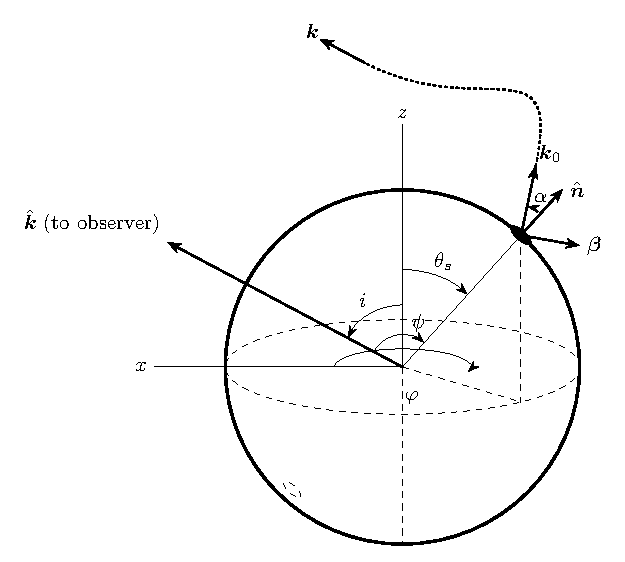
\includegraphics[width=0.85\columnwidth]{geometry_figure.pdf}
\caption{Geometry of the pulse-profile problem: the spot at colatitude $\theta_s$ on a star
    viewed at inclination $i$, the spot--observer angle $\psi$, and the photon's surface
    emission angle $\alpha$ (from the local normal $\hat{\boldsymbol{n}}$) bent onto the
    line of sight $\hat{\boldsymbol{k}}$; $\varphi$ is the rotational phase and
    $\boldsymbol{\beta}$ the spot's velocity. Redrawn after
    \citet{PoutanenBeloborodov2006}.\label{fig:geometry}}
\end{figure}
% fig:geometry is a native redraw (geometry_figure.tex) — no permission needed.
A single spot's flux can be defined as
\begin{equation}
F(\varphi) \propto \gamma\, B(\delta)\, D\, I(\mu')\, \mu' \cdot \mathbf{1}[\cos\alpha \ge
    0]. \label{eq:flux}
\end{equation}
We are basically chaining physical effects together; the comoving area ($\gamma$), Doppler
boost ($B$), gravitational solid-angle stretch (light-bending, $D$), surface brightness
($I$), and projection ($\mu' = \delta\cos\alpha$, the aberrated emission cosine, defined
with the rotation terms below). The flux is zero wherever the spot has set. Constants
(redshift powers, area, distance) are omitted, as they drop out of shapes and $\Delta
\mathrm{PF}$. On a frozen (non-rotating) star, $\gamma = B = 1$ and $\mu' = \cos\alpha$,
leaving $F \propto D\, I(\cos\alpha)\cos\alpha$ --- the static configuration behind our
headline numbers.
For light bending, we have implemented the Schwarzschild general-relativistic ray path
according to
\begin{equation}
\psi(\alpha) = \int_0^1 \frac{\tilde\beta\, dx}{\sqrt{1 - \tilde\beta^2 x^2 (1 - u x)}},
    \qquad \tilde\beta = \frac{\sin\alpha}{\sqrt{1-u}}, \label{eq:bending}
\end{equation}
with $D = d\cos\alpha / d\cos\psi$ evaluated numerically. {Here $\alpha$ is the photon's
emission angle at the star's surface and $u = 2GM/(Rc^2)$ the star's compactness.} This
bending is valid for $u < 2/3$, the compactness at which grazing light starts orbiting the
star, comfortably covering neutron-star simulations \citep{Pechenick1983}. All production
results use this exact map: at J0740's $u = 0.494$, the linear approximation of
\citet{Beloborodov2002} biased $\Delta \mathrm{PF}$ by $-0.0066$ and hid a $\sim$14\%
per-spot eclipse. (Both numbers come from re-running the identical anchor pipeline with the
linear map swapped back in; the run reproduces the earlier linear-bending branch
bit-for-bit, so the difference isolates the bending treatment alone.)

The rotation layer can switch on a special-relativistic setting, when considering spin
frequencies and stellar radii where the Doppler effect becomes non-negligible. Thus we need
to calculate how fast the spot moves and how that affects the photons (Doppler effect,
aberration).
The spot moves with surface speed
\begin{equation}
\beta = \frac{2\pi\nu R \sin\theta_s}{c\,\sqrt{1-u}}, \qquad \gamma =
    \frac{1}{\sqrt{1-\beta^2}}, \label{eq:speed}
\end{equation}
where $\nu$ is the spin frequency and $R$ the star's radius; the $\sqrt{1-u}$ is the
gravitational enhancement of the locally measured velocity (J0740 at 346.5\,Hz gives $\beta
\approx 0.12$). Each photon is then boosted by the Doppler factor
\begin{equation}
    \delta = \frac{1}{\gamma\,(1 - \beta\cos\xi)}, \label{eq:doppler}
\end{equation}
where $\xi$ is the angle between the photon direction and the spot velocity ($\delta > 1$
approaching, $\delta < 1$ receding). The same motion tilts the apparent emission angle
(aberration) giving the $\mu' = \delta\cos\alpha$ of Equation~\eqref{eq:flux}. Aberration is
why the beaming swap cannot ignore the Doppler Effect: it moves the $\mu$ at which $I(\mu)$
is sampled, so spin and the swap do not factor apart \citep{Bogdanov2019}.
When lumping all photon energies (bolometric), this is calculated as
\begin{equation}
B = \delta^{\,n}, \qquad n = 4\ (\text{energy flux})\ \text{or}\ 3\ (\text{photon flux}).
    \label{eq:boost}
\end{equation}
However, NICER uses an instrument band for their measurements, in this case we must use
\begin{align}
B &= \frac{\Phi_k(\delta)}{\Phi_k(1)}, \qquad k = 2\ (\text{counts})\ \text{or}\ 3\
    (\text{energy}), \nonumber \\
\Phi_k(\delta) &= \int_{E_1}^{E_2} \frac{E^k\, dE}{\exp\big[E / \big(\delta\sqrt{1-u}\,
    kT\big)\big] - 1}. \label{eq:bandboost}
\end{align}
Both utilize the Doppler factor $\delta$.
{Here $E$ is the photon energy, $[E_1, E_2]$ the instrument band (the band each J0740 fit
was calibrated on: 0.3--1.5\,keV for Riley, NICER channels [30, 150); 0.3--1.24\,keV for
Miller), and $kT$ the spot temperature in energy units; every Doppler and redshift factor
collapses into the single effective temperature $\delta\sqrt{1-u}\,kT$. A very wide band
recovers the bolometric $\delta^{3}/\delta^{4}$, but when the band sits on the exponentially
falling Wien tail of the spectrum (J0740's conditions) the boost is steeper than any power
of $\delta$.}

For stars with multiple hotspots, we sum single spot fluxes, weighing each by its area and
temperature accordingly:
\begin{equation}
F_\star(\varphi) = \sum_k w_k\, F(\varphi - \varphi_{0,k}), \qquad w_k \propto A_k\, T_k^4.
    \label{eq:spotsum}
\end{equation}
We then calculate a pulsed fraction by the function below, noting that whenever flux touches
0, it saturates at 1:
\begin{equation}
    \mathrm{PF} = \frac{F_{\max} - F_{\min}}{F_{\max} + F_{\min}}. \label{eq:pf}
\end{equation}
Lastly, we can compute the change in PF, running the identical chain twice --- once with the
library beaming and once with isotropic emission ($I \equiv 1$):
\begin{equation}
\Delta \mathrm{PF} = \mathrm{PF}\big[F_\star^{\text{realistic}}\big] -
    \mathrm{PF}\big[F_\star^{\text{isotropic}}\big]. \label{eq:dpf}
\end{equation}


\subsection{Validation} \label{sec:methods-validation}
The methodology was validated by comparing four central parts to academic work: the Monte
Carlo Scattering Atmosphere, the beaming curve, the Pulse-Profile machinery, and the Doppler
+ aberration layer. Figure~\ref{fig:validation} collects the three benchmark comparisons.

The Monte Carlo Scattering Atmosphere, when set to isotropic scattering, reproduces
Chandrasekhar's exact $H(\mu)$ solution, which models emergent radiation of an atmosphere
\citep{Chandrasekhar1960}. When comparing flux, reduced $\chi^2 = 0.70$ at $\tau = 10$, 5
seeds, $4.1\times10^5$ escaped. The comparison is made in flux space: the binned escape
counts (which measure $I(\mu)\,\mu$) are tested directly against $H(\mu)\,\mu$,
with Poisson counting errors on the pooled counts (the seed-to-seed
scatter sets the error bars in Figure~\ref{fig:validation}, not the $\chi^2$), over 17
degrees of freedom; the largest single-bin residual is $1.6\sigma$. Testing in flux space avoids the bin-center bias that unfolding to
intensity introduces at grazing angles. This means the transport engine (when using
isotropic scattering) is near-exact to Chandrasekhar.
One qualifier though, the transport engine uses Thomson scattering outside of this testing.
This sits around $\chi^2 = 1.49$, a $2.8\%$ maximum deviation to Chandrasekhar's isotropic
H.
{This 2.8\% is the measured phase-function sensitivity of the emergent beaming which is why
we describe the production atmosphere as \emph{near-exact} to $H(\mu)$, rather than exact.}

To verify the beaming curve extrapolated from the Monte Carlo, we fit to the limb-darkening
form: $I(\mu) = a(1+b\mu)$. Here we calculated $b = 1.79$,\footnote{The Thomson control in
Figure~\ref{fig:validation} (left) quotes $b = 1.72$ from that panel's independent
validation run and per-run unfolding; the $b = 1.79$ used throughout is the escape-matched
production library's pooled extraction, a $\sim 2\sigma$ (seed-scatter) difference, and
only the library curve feeds the pulse machinery.} which lies above both classical
thick-atmosphere predictions --- Eddington's approximate $b = 1.5$ and the $b \approx 1.68$
of Chandrasekhar's exact isotropic-scattering $H(\mu)$
\citep{Chandrasekhar1960,Mihalas1978}. The excess over $H(\mu)$ has the same origin as the
2.8\% phase-function sensitivity above: Thomson scattering limb-darkens slightly more
strongly than isotropic scattering. The resulting ordering, Eddington $<$ $H(\mu)$ $<$
Thomson slab ($1.50 < 1.68 < 1.79$), is put to work in Section~\ref{sec:discussion}, where
$\Delta$PF is shown to track $b$ monotonically (to within seed error)
across all three laws --- so no conclusion
hinges on which law is adopted.

We compared our pulse-profile machinery to Bogdanov's SD1a benchmark. Feeding in the
parameters set by the benchmark, our model is accurate to the benchmark up to
0.81\% when
considering linear bending, and 0.11\% when considering Schwarzschild bending
\citep{Bogdanov2019,Pechenick1983}. These residuals are the maximum pointwise difference
between the two waveforms after each is normalized to its own peak, quoted as a percentage
of the peak. The drop from 0.81\% to 0.11\% when the exact map replaces
the linear one is
itself evidence that the $\sim$1\% gap \emph{was} the linear approximation, not the pulse
machinery.

Lastly, we verified the Doppler and aberration layer against Bogdanov's SD1c benchmark,
which spins the SD1a geometry at 200\,Hz. The layer-enabled pulse profile machinery matches
the benchmark to max $|\Delta| = 1.35\%$ (same peak-normalized metric).
For this comparison the light-travel-time delay --- which the reference
waveform natively includes --- is switched on in our model, making the comparison
like-for-like; the remaining approximation
against the reference code is the linear bending map --- the residual is consistent with the
$\sim$1\% bending floor isolated in SD1a, rather than with any error in the rotation layer
itself. {As an extra cross-check, we re-derived the Doppler and aberration formulas through
a from-scratch 4-vector Lorentz boost, which agrees with the production implementation to
machine precision.}

\begin{figure*}[t]
    \centering
    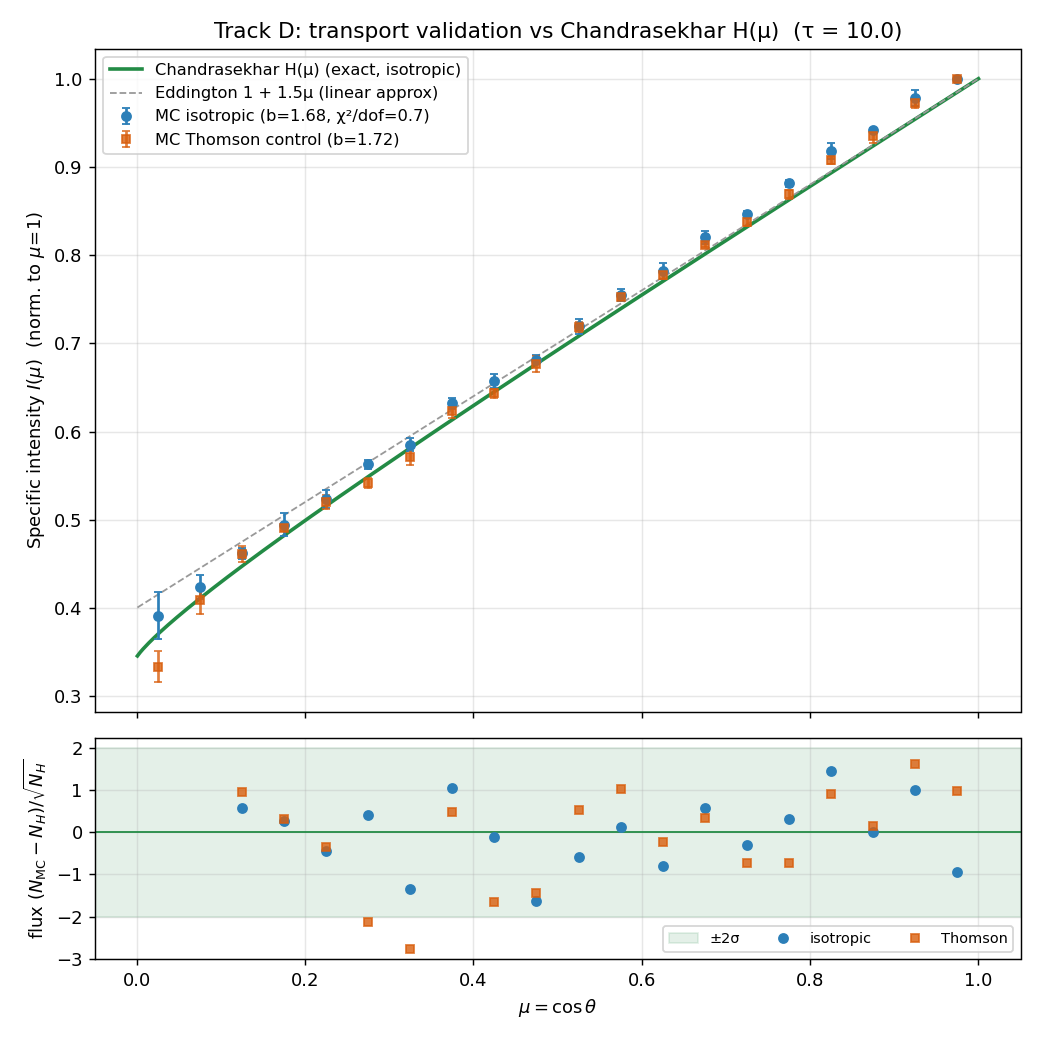
\includegraphics[width=0.32\textwidth]{d_isotropic_h_overlay.png}\hfill
    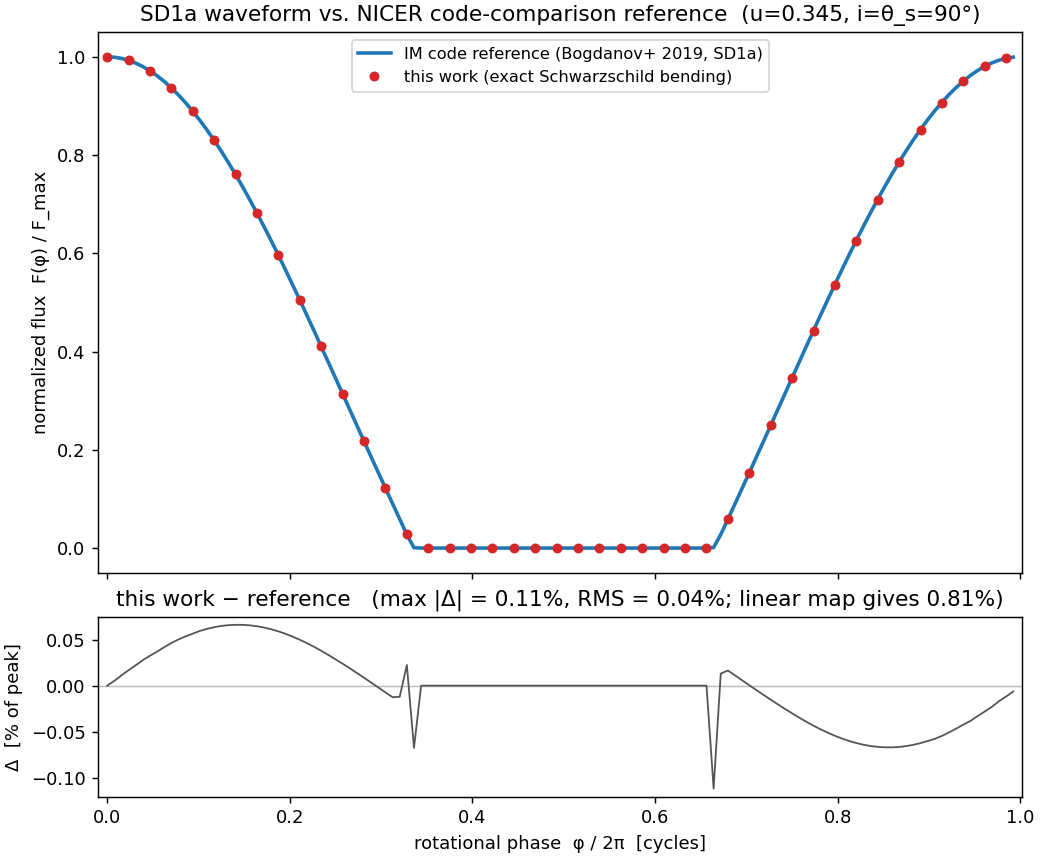
\includegraphics[width=0.32\textwidth]{pulse_profile_code_comparison.png}\hfill
    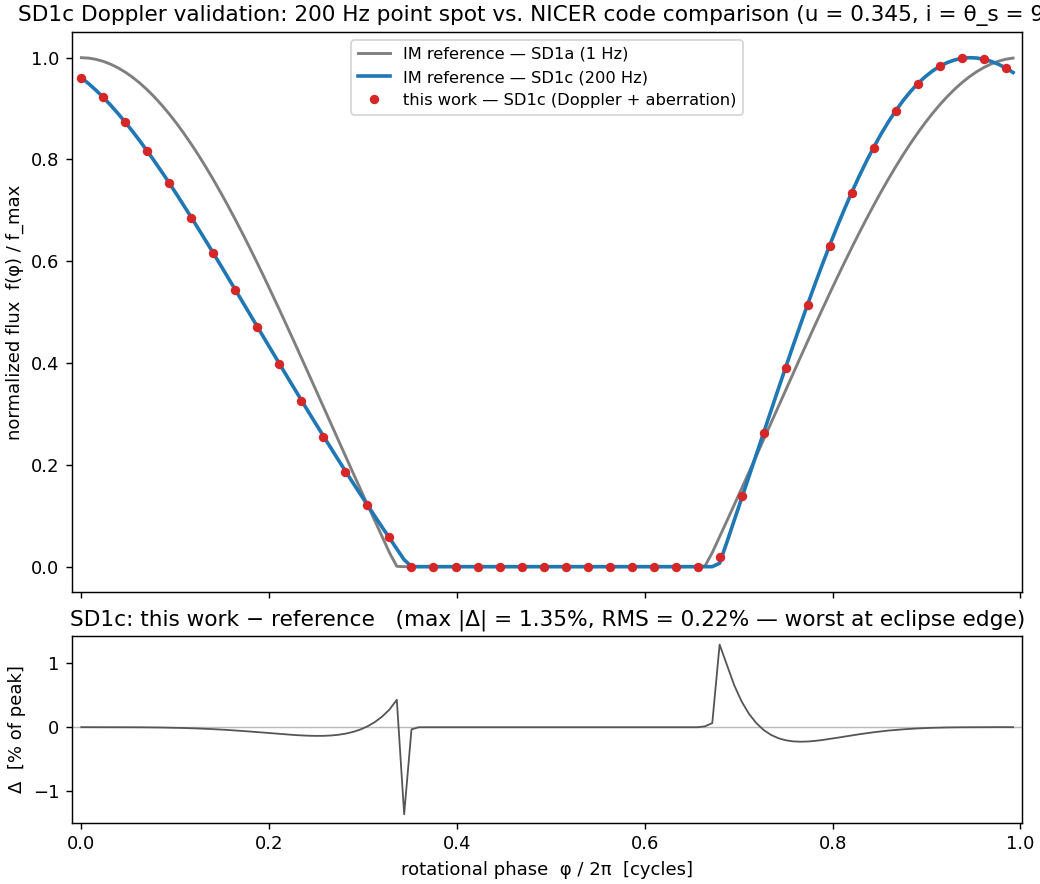
\includegraphics[width=0.32\textwidth]{pulse_profile_doppler_sd1c.png}
\caption{Validation gallery. \emph{Left:} the isotropic-mode Monte Carlo against
    Chandrasekhar's $H(\mu)$ in flux space (reduced $\chi^2 = 0.70$). \emph{Middle:} the
    static pulse machinery against the Bogdanov et al.\ SD1a reference waveform (max
    $|\Delta| = 0.11\%$ with exact bending). \emph{Right:} the rotation layer against the
    200\,Hz SD1c reference (max $|\Delta| = 1.35\%$).\label{fig:validation}}
\end{figure*}

This leads us to conclude that the random walk itself is right, the emergent brightness is
sensible, and the deterministic machinery matches independent benchmarks. 

\subsection{Target Configurations} \label{sec:methods-targets}
NICER has published 2 key measurements for neutron stars J0740 and J0030
\citep{Riley2019,Riley2021,Miller2019,Miller2021}. The geometries are referenced below.
Operationally, we are swapping these star's hotspots, between an equally bright hotspot
(isotropic) and a limb-darkened hotspot (realistic).
Each measurement comes in two independent fits (Riley and Miller). For J0740 they agree on
the star measurements but disagree on where the spots sit (opposite hemispheres vs.\
essentially on the equator). The geometry results are sensitive to this kind of uncertainty,
so we act on both. Table~\ref{tab:anchors} lists the fitted geometries. J0740 spins at
346.5\,Hz and is viewed nearly edge-on with two nearly anti-phased spots, meaning the
hotspots tile and summed flux never touches zero. J0030's spots both sit in the far
hemisphere, so their combined flux touches zero, the hotspots do not tile. The two anchors
therefore land on opposite sides of the criterion in Section~\ref{sec:results-tiling}.

\begin{deluxetable}{lcccc}
    \tablecaption{Anchor geometries from the published fits.\label{tab:anchors}}
\tablehead{\colhead{Fit} & \colhead{$i$} & \colhead{$\theta_s$ (spots)} &
    \colhead{$\Delta\varphi$ (cyc)} & \colhead{$u$}}
    \startdata
    J0740 Riley  & $87.6^\circ$ & $77^\circ,\ 108^\circ$   & $0.44$ & $0.494$ \\
    J0740 Miller & $87.5^\circ$ & $92^\circ,\ 92^\circ$    & $0.56$ & $0.444$ \\
    J0030 Riley  & $53.9^\circ$ & $128^\circ,\ 167^\circ$  & $0.45$ & $0.312$ \\
    J0030 Miller & $50.3^\circ$ & $130^\circ,\ 138^\circ$  & $0.46$ & $0.326$ \\
    \enddata
\tablecomments{$i$ = observer inclination, $\theta_s$ = spot colatitudes, $\Delta\varphi$ =
    azimuthal separation in rotation cycles, $u$ = compactness. Spot weights follow each
    paper's areas and temperatures ($w \propto A\,T^4$), except J0030
    Riley, whose crescent-shaped spots do not reduce cleanly to point-spot areas and share
    a single temperature; its two spots are weighted equally.}
\end{deluxetable}

\section{Results} \label{sec:results}

\subsection{Realistic Beaming Raises the Pulsed Fraction} \label{sec:results-pf}
Replacing the isotropic-emission assumption with a scattering-atmosphere makes the hot
spot's pulse sharper, raising its pulse fraction. For the J0740 geometry, the effect can be
seen directly in the pulsed fraction. Quantitatively, $\Delta\mathrm{PF} = +0.137 \pm 0.003$
(Riley fit) /
  $+0.195 \pm 0.005$ (Miller fit).
These are the static, bolometric numbers, with exact bending and the $\tau = 10$ atmosphere;
spin and the instrument band dilute them later (Section~\ref{sec:results-spin}), but the
systematic is cleanest here. The mechanism itself is simple: a limb-darkened hotspot is
brighter face-on and dimmer at grazing angles than an equally bright one, so its pulse peaks
higher and bottoms out lower --- a sharper pulse (Figure~\ref{fig:j0740}). The quoted errors
are seed-to-seed scatter of the Monte Carlo library. Nor does the headline depend on the
zero-background idealization: adding a common unpulsed background of up to 30\% of the
isotropic peak to both curves moves $\Delta$PF by less than $0.003$ --- within the seed
error --- because J0740's summed flux floor keeps the pulsed fraction well away from
saturation.

\begin{figure*}[t]
    \centering
    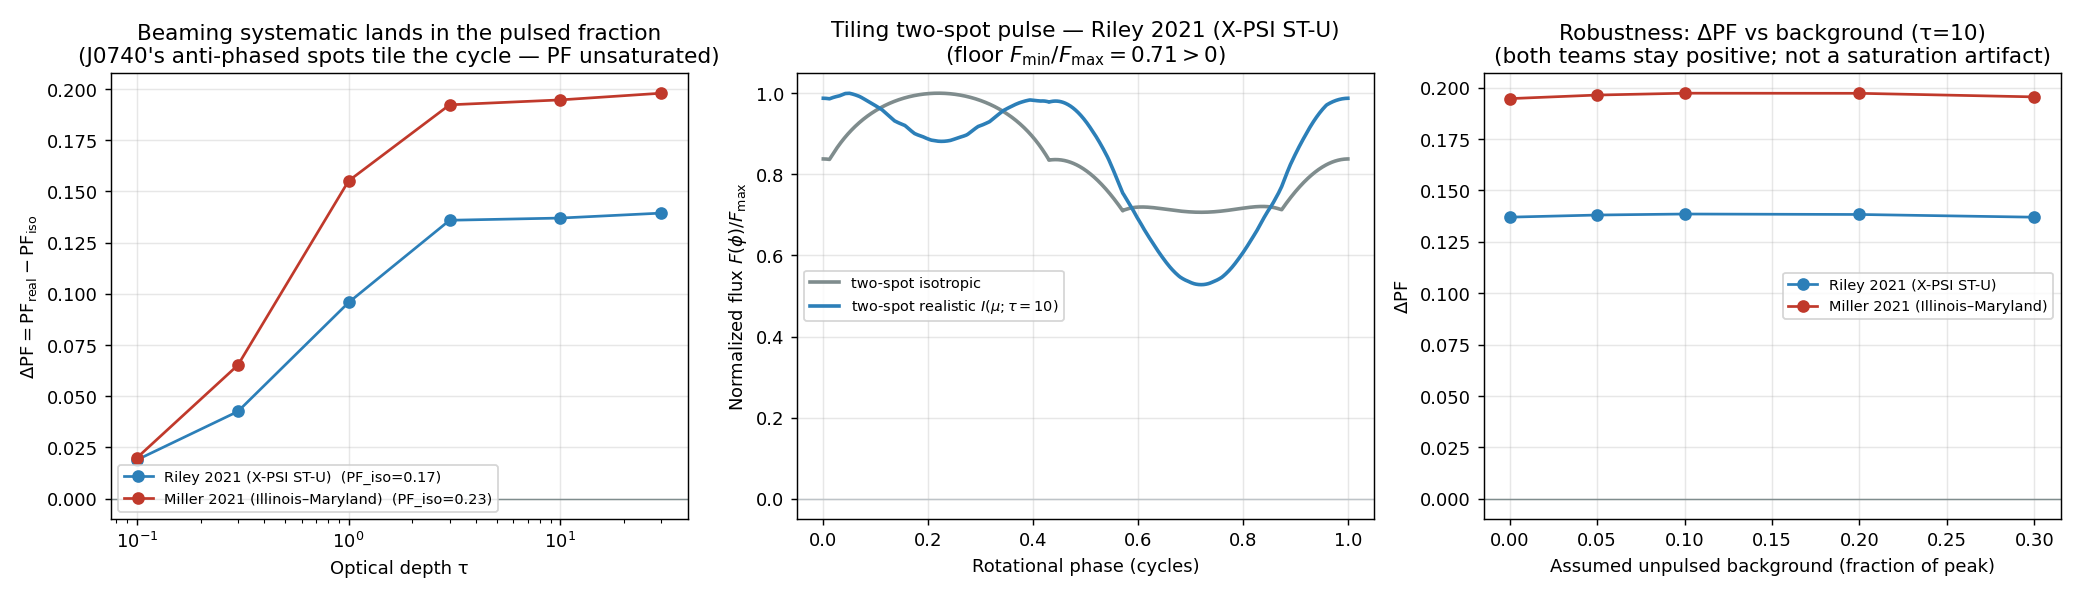
\includegraphics[width=\textwidth]{pulse_profile_j0740.png}
\caption{J0740 pulse profiles, isotropic vs.\ realistic beaming, for both published fits.
    The realistic curve peaks higher and dips lower --- the $\Delta$PF of
    Section~\ref{sec:results-pf}.\label{fig:j0740}}
\end{figure*}

\subsection{Geometry Routes the Systematic} \label{sec:results-routing}
Geometry decides whether the beaming systematic shows up in the pulsed fraction or hides in
the waveform shape.
The two anchors land on opposite sides of this divide. J0740's nearly anti-phased spots on a
nearly edge-on star keep at least one spot in view at every phase: the summed flux never
touches zero, the pulsed fraction stays unsaturated, and the systematic lands in $\Delta$PF
(the numbers above). J0030's spots both sit in the far hemisphere: the combined flux does
touch zero, the pulsed fraction pins at 1 for \emph{both} beamings, and $\Delta\mathrm{PF}
\approx 0$. The systematic does not disappear, but it moves into the waveform shape, where
the peak-normalized difference between isotropic and realistic curves is $\sim$6\% RMS
($0.061 \pm 0.002$ Riley, $0.058 \pm 0.001$ Miller; seed-to-seed) (Figure~\ref{fig:j0030}).
Throughout this paper the waveform-shape difference is defined by normalizing each curve to
its own peak, $\hat F = F/F_{\max}$, and taking the root-mean-square of the pointwise
difference over phase, $\big\langle (\hat F^{\text{real}} - \hat F^{\text{iso}})^2
\big\rangle_\varphi^{1/2}$. Because each curve is divided by its own peak, the metric is
insensitive to the pulsed fraction --- it keeps reading even where PF saturates, which is
exactly the regime that needs it.
The hard $\mathrm{PF} = 1$ saturation is the zero-background limit of the model. Real data
always carry unpulsed flux (instrumental background, emission from the rest of the surface),
which lifts the summed minimum off zero and un-saturates PF. Repeating the J0030 swap with a
common unpulsed background of 5--30\% of the isotropic peak added to both curves re-exposes
a positive PF systematic of $+0.03$ to $+0.14$, growing with the assumed level. Because that
level is an unconstrained knob we do not headline the re-exposed number; the point is that
saturation hides the systematic from the pulsed fraction only in the limit, while the
waveform-shape metric reads through at any background level.

\begin{figure*}[t]
    \centering
    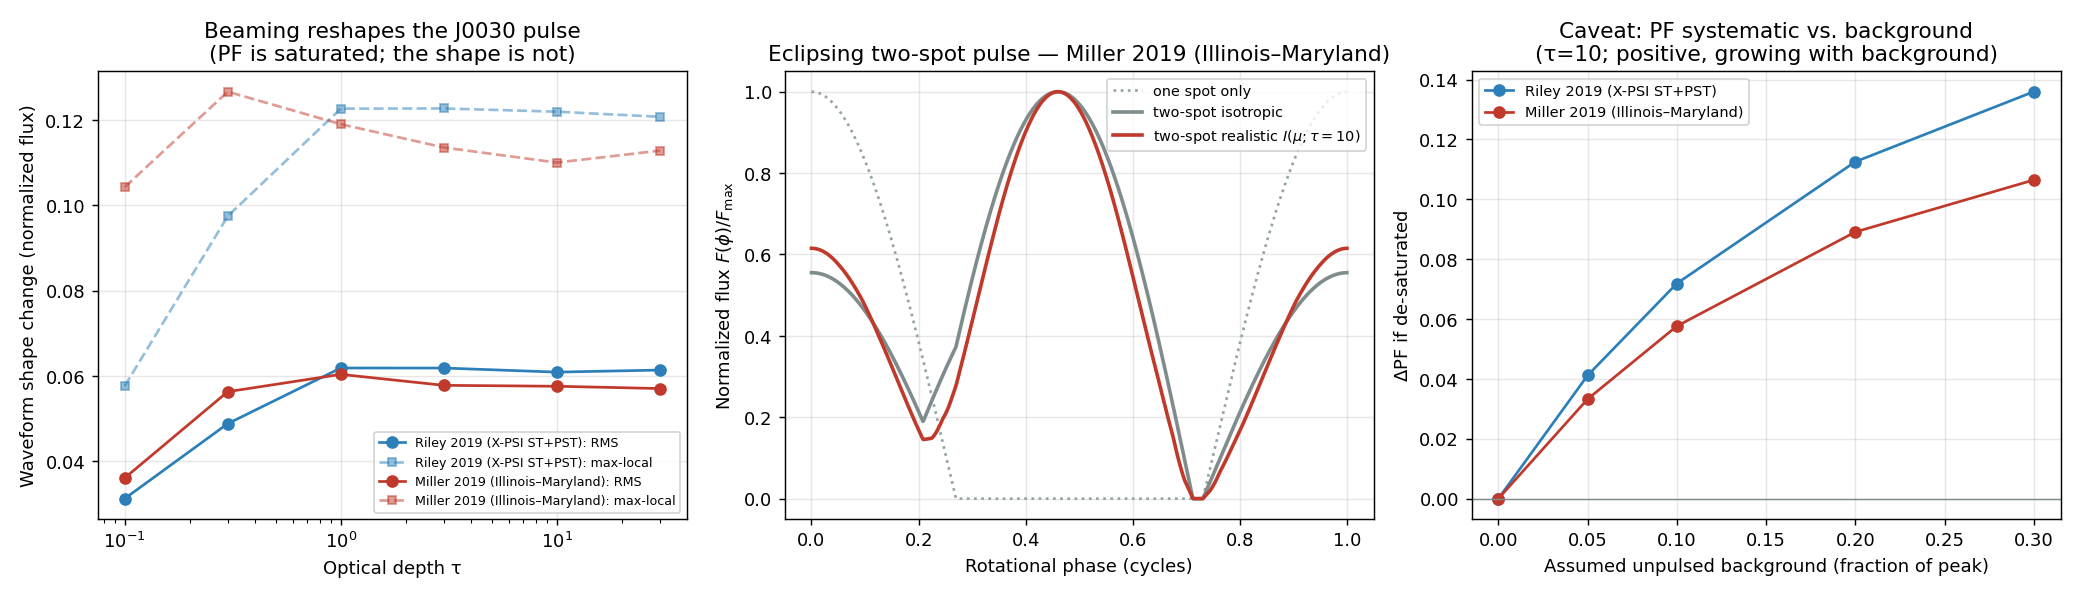
\includegraphics[width=\textwidth]{pulse_profile_j0030.png}
\caption{J0030 pulse profiles, isotropic vs.\ realistic beaming. The flux touches zero, so
    PF saturates at 1 for both curves and the systematic appears only in the waveform
    shape.\label{fig:j0030}}
\end{figure*}

\subsection{The Tiling Criterion} \label{sec:results-tiling}
The line between these two regimes is sharp, and it is a property of the \emph{summed} flux,
not of any single spot. The pulsed fraction saturates exactly when the combined multi-spot
flux of Equation~\eqref{eq:spotsum} touches zero at some phase (when the spots fail to tile
the rotation). Individual eclipses do not decide it: in the J0740 Miller fit, each spot is
hidden for $\sim$23\% of the cycle on its own, yet the anti-phased pair still tiles (the
summed flux floor is 0.63; 0.71 for the Riley fit) and the pulsed fraction stays live. A
single spot never fully sets while $\cos(i+\theta_s) \ge -u/(1-u)$ --- the threshold is
negative because light bending lets us see past the geometric limb --- but the criterion
that matters applies to the spot sum, not to each spot individually. (The threshold follows
from the linear bending map $\cos\alpha \approx u + (1-u)\cos\psi$ evaluated at the spot's
farthest swing, $\cos\psi = \cos(i+\theta_s)$: the spot remains visible while some surface
emission angle can reach the observer, $\cos\alpha \ge 0$, which rearranges to the stated
condition. The numbers quoted for the Miller fit --- the $\sim$23\% per-spot eclipse and the
0.63 summed-flux floor --- are computed directly from the Table~\ref{tab:anchors} geometry
with exact bending.) Figure~\ref{fig:phasediagram} maps the two regimes across geometry,
with azimuthal separation as an explicit axis: the regime boundary is analytic, and every
configuration we ran falls on the side the criterion predicts.
The linear map's only role is to draw that analytic boundary; the regime assignments never
rely on it. The $\Delta$PF map itself is computed with the full numerical engine, whose
eclipse onset reproduces the analytic condition exactly across the grid, and the two anchors
are re-evaluated with exact bending --- which at J0740's $u = 0.494$ exposed the $\sim$14\%
Riley per-spot eclipse yet moved no configuration across the boundary (the floors above are
exact-bending values). Exact bending sharpened the criterion; it did not relocate it.

\begin{figure*}[t]
    \centering
    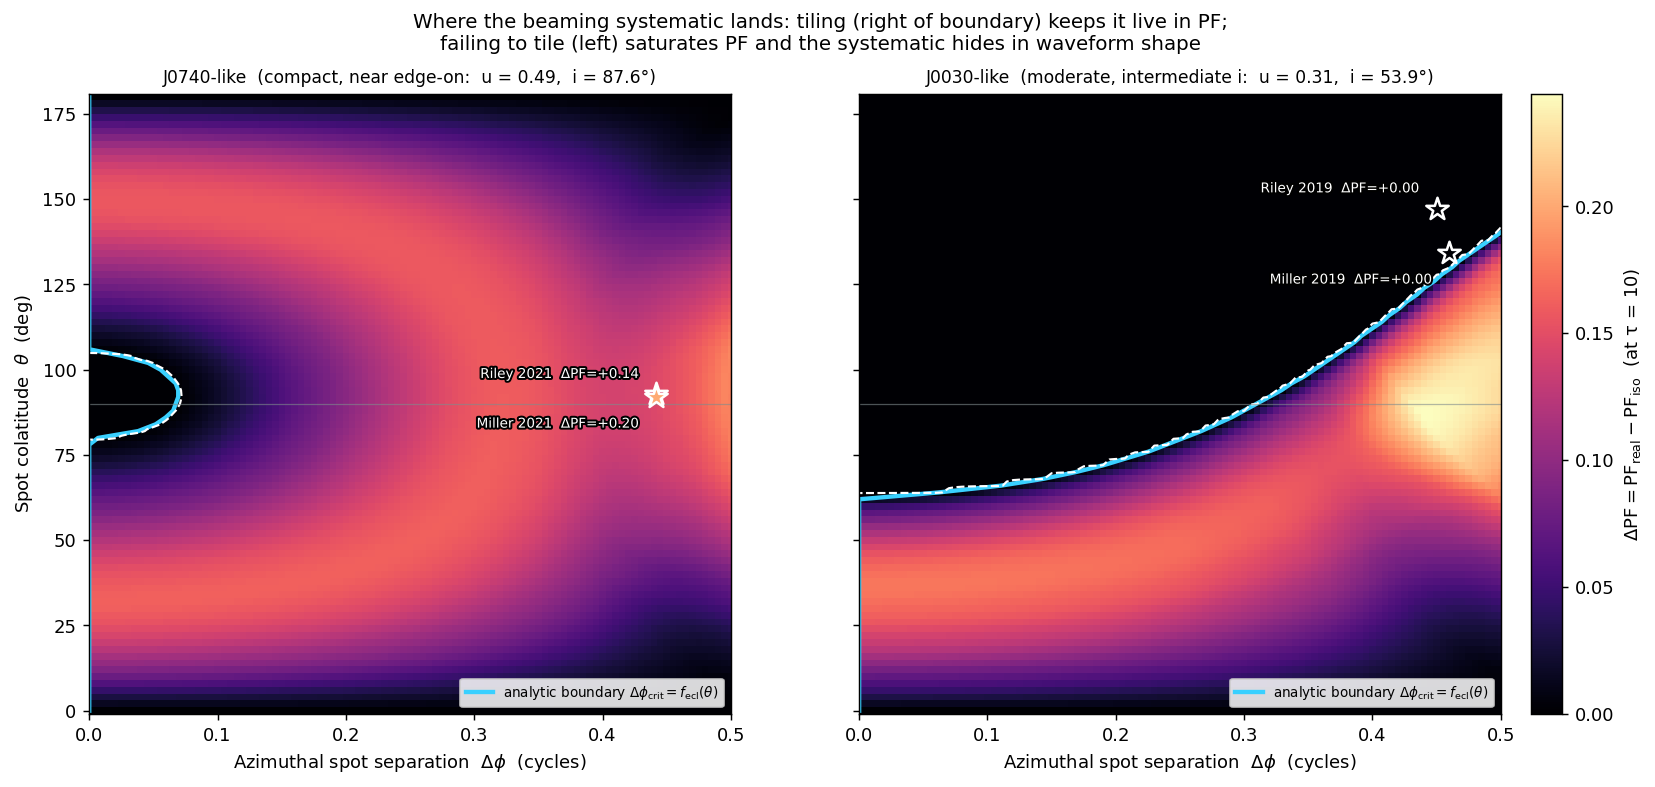
\includegraphics[width=0.85\textwidth]{phase_diagram.png}
\caption{Phase diagram of the beaming systematic's routing. Geometries that tile the
    rotation keep the pulsed fraction live (systematic in $\Delta$PF); geometries that do
    not tile saturate PF at 1 and route the systematic into waveform
    shape.\label{fig:phasediagram}}
\end{figure*}

\subsection{Spin Drains the Pulsed Fraction but Not the Shape} \label{sec:results-spin}
At the real spin, the story changes --- but only for the pulsed fraction. At 346.5\,Hz the
Doppler boost pumps a large second harmonic (a twice-per-rotation component) into
\emph{both} the isotropic and realistic curves. The harmonic arises from the pairing: each
spot's Doppler boost is a once-per-rotation modulation that peaks as that spot approaches
the observer, and for two nearly anti-phased spots those peaks land half a cycle apart, so
their sum carries strong twice-per-rotation power. This shared signal saturates the min/max
statistic of Equation~\eqref{eq:pf}, so the PF systematic drains: from $+0.137$/$+0.195$
static down to a residual of $+0.02$ to $+0.07$, depending on the boost convention and
instrument band (Table~\ref{tab:ladder}). The waveform-shape difference does not drain. The
peak-normalized RMS difference holds at $\approx 0.10$ across spin, band, and light-travel
warp, and most of the fundamental-harmonic gap --- $\Delta(A_1/A_0)$, the once-per-rotation
amplitude relative to the mean --- survives, moving only from $+0.033$ to $+0.029$. The
systematic moves; it does not vanish. Quoting the spinning PF residual alone would read as
``the effect disappears,'' when in reality it relocates into observables that the pulsed
fraction cannot see (Figure~\ref{fig:ladder}).

\begin{figure}[t]
    \centering
    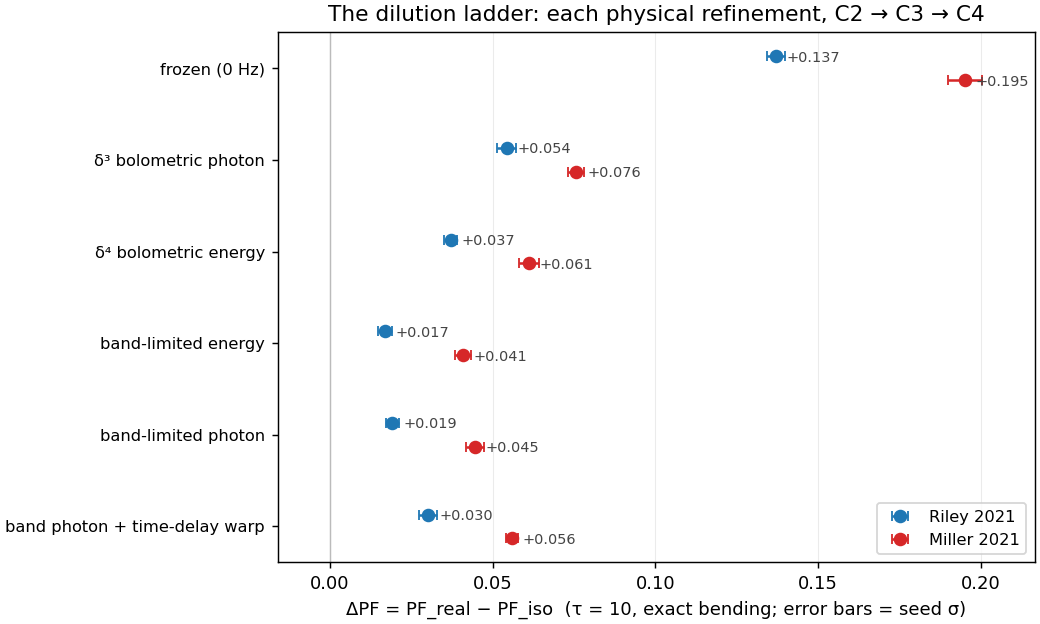
\includegraphics[width=\columnwidth]{doppler_dilution_ladder.png}
\caption{The $\Delta$PF dilution ladder: each rung adds one physical effect (spin, band,
    light-travel geometry) to the static baseline. The PF systematic drains while the shape
    difference holds.\label{fig:ladder}}
\end{figure}

% ---- Dilution-ladder table (numbers from claims-evidence.md A4) ------
\begin{deluxetable}{lcc}
    \tablecaption{$\Delta$PF dilution ladder for J0740.\label{tab:ladder}}
    \tablehead{\colhead{Configuration} & \colhead{Riley} & \colhead{Miller}}
    \startdata
    0 Hz static, bolometric              & $+0.137$ & $+0.195$ \\
    346.5 Hz, bolometric $\delta^4$      & $+0.037$ & $+0.061$ \\
    346.5 Hz, NICER-band photons         & $+0.019$ & $+0.045$ \\
    346.5 Hz, all geometry, $\delta^4$   & $+0.041$ & $+0.069$ \\
    346.5 Hz, all geometry, band photons & $+0.030$ & $+0.056$ \\
    \enddata
\tablecomments{Rows 2--3 add spin with the bolometric ($\delta^4$) and NICER-band
    photon-count boosts respectively; rows 4--5 repeat both with the full geometric terms
    (light-travel warp) included. The spread across rows is the convention dependence behind
    the quoted $+0.02$ to $+0.07$ range.}
\end{deluxetable}

\section{Discussion} \label{sec:discussion}
Relative to prior work, our contribution is the routing, not just the size.
\citet{Zhao2024a, Zhao2024b} showed that a wrong beaming function biases the inferred radius
through the fundamental-harmonic ratio $A_1/A_0$, and \citet{Baubock2015} quantified the
companion effect on inferred spot size. We show that \emph{where} the beaming systematic
appears --- pulsed fraction or waveform shape --- is itself decided by geometry and spin,
governed by the tiling criterion. The two views are complementary: when the spots tile, a
single number ($\Delta$PF) carries the systematic; when they do not, only shape observables
do.

Several limitations should be kept in mind. The atmosphere is a grey
(frequency-independent), passive, plane-parallel scattering slab at fixed $\tau = 10$ ---
deliberately simple, so that the isotropic-vs-realistic swap is the only moving part. It is
not a fitted atmosphere model: there are no energy-dependent opacities and no temperature
structure. In particular it is not the beamed hydrogen atmosphere (e.g. NSX, NSATMOS) that
the NICER pipelines fit; those atmospheres are likewise limb-darkened, so the sign and
geometry-routing carry over, but the band-exact magnitude against a fitted atmosphere is
future work. The transport engine is near-exact against $H(\mu)$ only in its
isotropic-scattering mode; the production Thomson curve differs from $H$ by up to 2.8\% (the
phase-function sensitivity). That said, the magnitude of $\Delta$PF tracks the
limb-darkening slope $b$ across different atmosphere laws, so the effect is a property of
limb darkening in general, not of our particular slab. (We repeated the full anchor analysis
with the slab replaced by the two classical analytic laws: Eddington's $b = 1.50$ and
Chandrasekhar's $H(\mu)$ with $b = 1.68$, alongside the Thomson slab's $b = 1.79$. All three
give a positive, PF-live static $\Delta\mathrm{PF}$ of $+0.128$ to $+0.196$, diluting to
$+0.026$ to $+0.061$ at 346.5\,Hz, with shape RMS 0.10--0.13 throughout --- and the
magnitudes are ordered by $b$ to within seed error (one static cell inverts
the $H(\mu)$--Thomson order by $0.0008$, $\approx 0.2\sigma$).) Light-travel delay \citep{Poutanen2020} and oblateness
($\sim$3\% at 346.5\,Hz \citealp{AlGendyMorsink2014}) are beaming-independent; including the
full light-travel geometry moves the spinning residual only within the range quoted in
Table~\ref{tab:ladder}. Our fluxes also carry no unpulsed background;
Sections~\ref{sec:results-pf} and \ref{sec:results-routing} show the J0740 headline is
insensitive to one and that at J0030 a background un-saturates PF and re-exposes (rather
than erases) the systematic, so the omission is conservative. Finally, the spinning PF
residual is convention-dependent ($\delta^3$ vs.\ $\delta^4$ vs.\ band), which is exactly
why we quote a range and not a single number.

The implication for measurement is direct. Analyses that lean on the pulsed fraction alone
--- quick estimates, sensitivity forecasts, population arguments
\citep[e.g.][]{AnnalaPoutanen2010,Psaltis2014,Sotani2018} --- inherit a beaming systematic
that can be large ($+0.14$ to $+0.20$ static), small ($+0.02$ to $+0.07$ at speed), or
entirely invisible (saturated), depending on geometry and spin. The waveform-shape
difference is the robust observable: it survived every configuration we tested.

\section{Conclusions} \label{sec:conclusions}
We measured the cost of the isotropic-emission shortcut in pulse-profile work, and found it
is not one number --- it is a systematic that moves. Three results summarize this paper.
First, replacing isotropic emission with a scattering-atmosphere beaming function sharpens
the pulse: at the published J0740 geometries, the pulsed fraction rises by $+0.137 \pm
0.003$ (Riley) to $+0.195 \pm 0.005$ (Miller) in the static, bolometric case. Second,
geometry decides where this systematic appears. If the hotspots tile the rotation (their
summed flux never touches zero), it lands in the pulsed fraction; if they do not, the pulsed
fraction saturates at 1 and the systematic hides in the waveform shape. The criterion
belongs to the spot \emph{sum} --- individual eclipses do not decide it. Third, spin is a
second router: at 346.5\,Hz the Doppler-driven second harmonic drains the PF residual to
$+0.02$--$+0.07$, while the waveform-shape difference ($\approx 0.10$ RMS) is nearly
spin-invariant. The systematic never vanishes --- it only moves outside whichever statistic
is being measured.

Natural next steps are an energy-dependent atmosphere, adding oblateness, and propagating
the shape-level difference through a full inference pipeline to a radius bias.

% =====================================================================
%  BACK MATTER — MDPI Universe requires every block below.
%  (AASTeX has no native commands for these; \section* is fine for the
%  draft. They map 1:1 onto fields in the MDPI template at revision.)
% =====================================================================

\section*{Author Contributions}
% MDPI wants CRediT taxonomy in their phrasing style. Draft:
Conceptualization, A.P. and A.u.-D.; Methodology, A.P.; Software, A.P.;
Validation, A.P.; Formal Analysis, A.P.; Investigation, A.P.;
Writing -- Original Draft Preparation, A.P.; Writing -- Review \&
Editing, A.u.-D.; Visualization, A.P.; Supervision, A.u.-D.

\section*{Funding}
This research was supported by the Multi-Campus Research Experiences for Undergraduates
(REU) program of The Pennsylvania State University.

\section*{Data Availability Statement}
The source code and simulation outputs supporting this study are
openly available on Zenodo at [DOI], archived from
https://github.com/Ameya-bit/mc-radiative-transfer.

\begin{acknowledgments}
% MDPI GenAI-use statement (required if AI assisted beyond grammar-level editing).
During the preparation of this manuscript, the author(s) used Claude Opus 4.8 for
code generation. The authors have reviewed and edited the output and take full
responsibility for the content of this publication.
\end{acknowledgments}

\section*{Conflicts of Interest}
The authors declare no conflicts of interest.


% ---- Facilities / software (optional AAS conventions) ----------------
% \facilities{NICER}
% \software{NumPy \citep{numpy}, Matplotlib \citep{matplotlib}}

% =====================================================================
%  REFERENCES  (BibTeX -> entries live in refs.bib)
% =====================================================================
%  Build order:  pdflatex -> bibtex -> pdflatex -> pdflatex
%  Only \cite'd entries appear, so refs.bib's "deferred" references stay
%  dormant until you cite them. To preview the whole database, temporarily
%  add \nocite{*} above \bibliography.
% While drafting: \nocite{*} renders ALL refs.bib entries even before any
% \cite appears in the text (also silences bibtex's "no \citation commands"
% error). Removed now that real citations exist, so only cited works print.
% \nocite{*}
\bibliographystyle{aasjournalv7}  % v6.31 uses "aasjournal" (no v7 suffix)
\bibliography{refs}

\end{document}
